
\begin{figure}[H]
  {
    \setlength{\tabcolsep}{3.0pt}
    \setlength\cmidrulewidth{\heavyrulewidth} % Make cmidrule = 
    \begin{adjustbox}{height=5cm,center}
      \footnotesize
      \begin{tabular}{ll}

        \makecell[l]{
\icode{.BYTE \$FF}\\
\icode{.BYTE \$FF}
} & \makecell[l]{
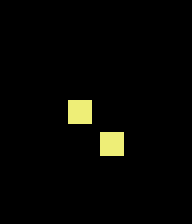
\includegraphics[width=1.3cm]{src/patterns/pixels/pixel_pattern3_0.png}%
} \\
        \midrule

        \makecell[l]{
\icode{.BYTE \$00}\\
\icode{.BYTE \$FE}
} & \makecell[l]{

\includegraphics[width=1.3cm]{src/patterns/pixels/pixel_pattern3_1.png}%
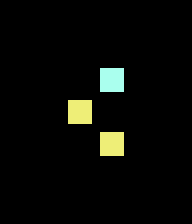
\includegraphics[width=1.3cm]{src/patterns/pixels/pixel_pattern3_2.png}%
} \\
        \midrule

        \makecell[l]{
\icode{.BYTE \$02}\\
\icode{.BYTE \$FF}
} & \makecell[l]{

\includegraphics[width=1.3cm]{src/patterns/pixels/pixel_pattern3_3.png}%

\includegraphics[width=1.3cm]{src/patterns/pixels/pixel_pattern3_4.png}%
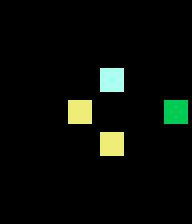
\includegraphics[width=1.3cm]{src/patterns/pixels/pixel_pattern3_5.png}%
} \\
        \midrule

        \makecell[l]{
\icode{.BYTE \$01}\\
\icode{.BYTE \$02}
} & \makecell[l]{
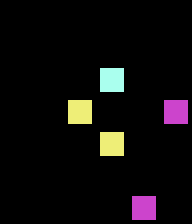
\includegraphics[width=1.3cm]{src/patterns/pixels/pixel_pattern3_6.png}%
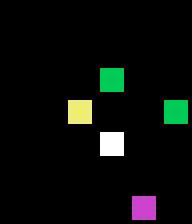
\includegraphics[width=1.3cm]{src/patterns/pixels/pixel_pattern3_7.png}%

\includegraphics[width=1.3cm]{src/patterns/pixels/pixel_pattern3_8.png}%
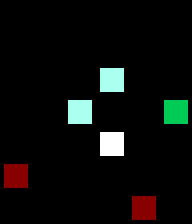
\includegraphics[width=1.3cm]{src/patterns/pixels/pixel_pattern3_9.png}%
} \\
        \midrule

        \makecell[l]{
\icode{.BYTE \$FD}\\
\icode{.BYTE \$01}
} & \makecell[l]{
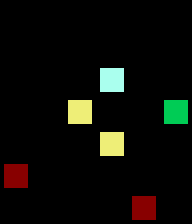
\includegraphics[width=1.3cm]{src/patterns/pixels/pixel_pattern3_10.png}%
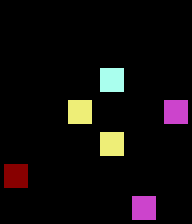
\includegraphics[width=1.3cm]{src/patterns/pixels/pixel_pattern3_11.png}%
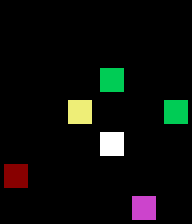
\includegraphics[width=1.3cm]{src/patterns/pixels/pixel_pattern3_12.png}%
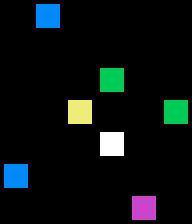
\includegraphics[width=1.3cm]{src/patterns/pixels/pixel_pattern3_13.png}%
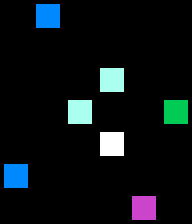
\includegraphics[width=1.3cm]{src/patterns/pixels/pixel_pattern3_14.png}%
} \\
        \midrule

        \makecell[l]{
\icode{.BYTE \$FE}\\
\icode{.BYTE \$FC}
} & \makecell[l]{
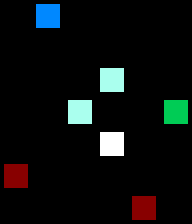
\includegraphics[width=1.3cm]{src/patterns/pixels/pixel_pattern3_15.png}%
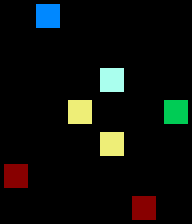
\includegraphics[width=1.3cm]{src/patterns/pixels/pixel_pattern3_16.png}%
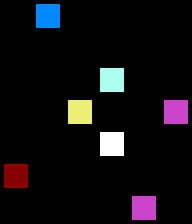
\includegraphics[width=1.3cm]{src/patterns/pixels/pixel_pattern3_17.png}%
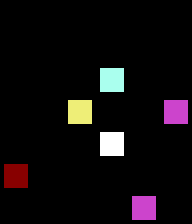
\includegraphics[width=1.3cm]{src/patterns/pixels/pixel_pattern3_18.png}%
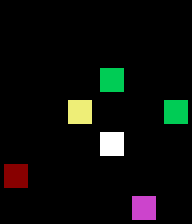
\includegraphics[width=1.3cm]{src/patterns/pixels/pixel_pattern3_19.png}%
} \\
        \midrule

        \makecell[l]{
\icode{.BYTE \$00}\\
\icode{.BYTE \$00}
} & \makecell[l]{
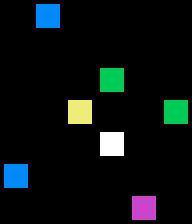
\includegraphics[width=1.3cm]{src/patterns/pixels/pixel_pattern3_20.png}%
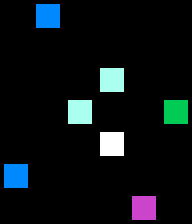
\includegraphics[width=1.3cm]{src/patterns/pixels/pixel_pattern3_21.png}%
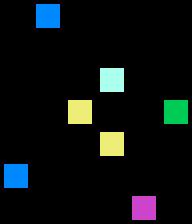
\includegraphics[width=1.3cm]{src/patterns/pixels/pixel_pattern3_22.png}%
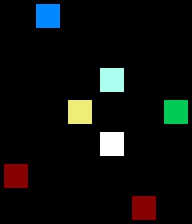
\includegraphics[width=1.3cm]{src/patterns/pixels/pixel_pattern3_23.png}%
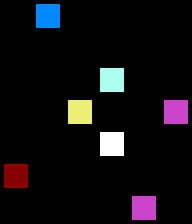
\includegraphics[width=1.3cm]{src/patterns/pixels/pixel_pattern3_24.png}%
} \\
        \midrule

      \end{tabular}
    \end{adjustbox}
  }\caption{The purpose of each of the oscillator values.}
\end{figure}
